\documentclass[11pt]{article}
\usepackage[a4paper,margin=1.8cm]{geometry}
\usepackage{amsmath, amssymb, amsthm}  % Essential math packages
\usepackage{graphicx}                   % For figures
\usepackage{hyperref}                   % Clickable links
\usepackage{parskip} % cleaner spacing
\usepackage{enumitem}
\usepackage{mdframed}
\usepackage{caption}     % For better captions
\usepackage{subcaption}  % For side-by-side figures
\usepackage{float}       % For [H] option (force placement)

% Define a solution environment with a box
\newenvironment{solbox}
  {\begin{mdframed}[linewidth=1pt,linecolor=black,roundcorner=5pt]
   \noindent\textbf{Ans: }\enspace}
  {\end{mdframed}}

\newcommand{\norm}[1]{\left \lVert #1 \right \rVert}
\newcommand{\compconj}[1]{%
  \overline{#1}%
}

\title{Oblig 3 \\ MAT1125 - Lineær Algebra}
\author{Oliver Ekeberg}
\date{\today}

\begin{document}
\maketitle


\tableofcontents


\section{3.5}

\subsection{3.5.8}

\begin{solbox}

    Vet allerede at $ A_{jk} \neq 0 $ for $ j=k $. Så antar bare en liste $ \left( A \right) _{jj} $ for $ j=1,..., min(m,n) $ 
    Fra definisjonen av matrisenormen er 

    \[
        \norm{A}_\mathcal{L} = sup_{x \in \mathcal{ K } ^n ,\norm{x}=1} \norm{Ax}_{l^2}
    \]

    fra thm 3.5.6 er $ \norm{Ax}_{l^2} \leq \norm{A}_\mathcal{L}  \norm{x}_{l^2}$
    
    Og siden 

    \[
        \norm{A}_{ \mathcal{L}}^{} := sup_{x \in \mathbb{K}^n, x \neq 0} \frac{ \norm{Ax}_{l^2}^{} }{ \norm{x}_{l^2}^{} } = sup_{x \in \mathbb{K}^n, \norm{x}_{}^{} =1} \norm{Ax}_{l^2}^{} 
    \]
    
    Vi kan da skrive om 

    \begin{align*}
        \norm{A}_{ \mathcal{L}}^{} \leq sup_{x \in \mathbb{K}^n, \norm{x}_{}^{} =1} \norm{A}_{ \mathcal{L}}^{} \norm{x}_{l^2}^{} =  sup_{x \in \mathbb{K}^n, \norm{x}_{}^{} =1} \norm{A}_{ \mathcal{L}}^{}
    \end{align*}

    Da må $ \norm{A}_{ \mathcal{L}}^{}  = max_j \left| \left( A \right)_{j,j}  \right|  $ 
    

\end{solbox}


\section{4.1}

\subsection{4.1.2}

\subsubsection{a)}

\begin{solbox}
    \begin{align*}
        \langle u, v+w \rangle &= \compconj{\langle v+w, u \rangle} \\
        &= \compconj{ \langle v, u \rangle } + \compconj{ \langle w, u \rangle } \\
        &= \langle u, v \rangle + \langle u, w \rangle 
    \end{align*}
    Som viser at egenskap 2 for indreprodukt er additiv

\end{solbox}


\subsubsection{b)}

\begin{solbox}
    \begin{align*}
        \langle u, \alpha  v\rangle &= \compconj{ \langle \alpha_{}^{} v, u \rangle } \\
        &= \compconj{ \alpha_{}^{} \langle v, u \rangle } \\
        &= \compconj{\alpha_{}^{} } \langle u, v \rangle 
    \end{align*}


    
\end{solbox}

\subsubsection{c)}
\begin{solbox}
    Om $ \mathbb{K} = \mathbb{R} $ så er indreproduktet om $ x, y \in \mathbb{R} $ lik
    
    \begin{align*}
        \langle x, y \rangle &= x * y \\
        &= \sum_{ j=1 }^{ n } x_j * y_j \\
        &= \sum_{ j=1 }^{ n } y_j * x_j \\
        &= y * x \\
        &= \langle y, x \rangle 
    \end{align*}
    


\end{solbox}

\subsection{4.1.3}

\begin{solbox}
    Vet at $ u \in U $ og at $ \langle u, v \rangle =0 $ for den utvalgte u $ \forall v \in U $. Skal først vise at $ u=0 $.
    
    
    $ \forall v \in U$, $ \exists u \in U $ s.a. $ v=u $. Siden $ \langle u, v \rangle =0 \forall v \in U $, så må $ \langle u,u \rangle = 0$. Fra første egenskap av indreproduktrom vet vi at
    
    \[
        \langle u, u \rangle =0 \Longleftrightarrow u=0
    \]

    Og vi har vist at $ u=0 $.
    
    
    Spørsmålet er nå om det samme gjelder dersom $ \langle v, u \rangle =0 $ for alle $ v \in U $.
    
    
    \begin{align*}
        \langle v, u \rangle &= \compconj{ \langle u, v \rangle }
    \end{align*}

    Siden $ 0 = \compconj{0} $ , så er $ \langle v, u \rangle = \compconj{0}  =0$. Det kommer av at $ \langle u, v \rangle =0 $ som vi allerede har vist
    
    
\end{solbox}


\subsection{4.1.5}


\begin{solbox}
    Vi har det kanoniske prikkproduktet for $ \mathbb{K}^n $ 

    \[
        \langle x, y \rangle _{\mathbb{K}^n} := x^T \compconj{y} = \sum_{ k=1 }^{ n } x_k \compconj{y}_k
    \]

    Skal nå vise at det er et prikkprodukt. Da må det tilfredsstille i)-iv)

    \begin{enumerate}
        \item \begin{align*}
            \langle x, x \rangle = x^T \compconj{x} = \sum_{ k=1 }^{ n } x_k \compconj{x}_k
        \end{align*}
         
        som er $ \geq 0 $ og $ =0 \Longleftrightarrow x=0$  
        \item for en $ z \in \mathbb{K}^n $ er  \begin{align*}
            \langle x+y, z \rangle &= \sum_{ k=1 }^{ n } (x+y)_k \compconj{z}_k \\
            &= \sum_{ k=1 }^{ n } x_k \compconj{z}_k + y_k \compconj{z}_k \\
            &= \langle x, z \rangle + \langle y, z \rangle 
        \end{align*}

        \item for en $ a \in \mathbb{K} $ er \begin{align*}
            \langle ax, y \rangle &= \sum_{ k=1 }^{ n } ax_k \compconj{y}_k \\
            &= a \sum_{ k=1 }^{ n } x_k \compconj{y}_k \\
            &= a \langle x, y \rangle 
        \end{align*}

        \item \begin{align*}
            \langle x, y \rangle &= \sum_{ k=1 }^{ n } x_k \compconj{y}_k \\
            &= \sum_{ k=1 }^{ n } \compconj{y}_k x_k \\
            &= \sum_{ k=1 }^{ n } \overline{ y_k \overline{x_k}}\\
            &= \compconj{\langle y, x \rangle}  
        \end{align*}
        
    \end{enumerate}
    Og jeg har vist at $ \langle x, y \rangle _{\mathbb{K}^n} $ er et indreproduktrom 
\end{solbox}

\subsubsection{c)}

\begin{solbox}
    Vi har l2 rommet $\ell^2(\mathbb{K}) := 
    \left\{ (a_1, a_2, \ldots) \; : \; 
    \sum_{k \in \mathbb{N}} |a_k|^2 < \infty 
    \right\}$. Vi definerere så $ \ell^2 $ indreproduktet som 

    \[
        \langle a, b \rangle _{\ell^2} := \sum_{ k=1 }^{ \infty } a_k \overline{b}_k
    \]
    Skal nå vise at dette er et indreproduktrom

    \begin{enumerate}
        \item \begin{align*}
            \langle a, a \rangle _{\ell^2} = \sum_{ k=1 }^{ \infty } a_k \overline{a}_k
        \end{align*}
        Og dette er åpenbart $ \geq 0 $ og $ =0 \Longleftrightarrow a_k=0 \forall k=1,2,...$  

        \item for en $ c = \left( c_1, c_2, ... \right) \in \ell^2 (\mathbb{K}) $ så er
        
        \begin{align*}
            \langle a+b, c \rangle _{\ell^2} &= \sum_{ k=1 }^{ \infty } \left( a + b \right) _k \overline{c}_k \\
            &= \sum_{ k=1 }^{ \infty } \left( a_k + b_k \right) \overline{c}_k \\
            &= \sum_{ k=1 }^{ \infty } a_k \overline{c}_k + b_k \overline{c}_k \\
            &= \langle a, c \rangle _{\ell^2} + \langle b, c \rangle _{\ell^2}
        \end{align*}

        \item for en $ \alpha_{}^{} \in \mathbb{K} $ så er  \begin{align*}
            \langle \alpha_{}^{} a, b \rangle_{ \ell^2 } &= \sum_{ k=1 }^{ \infty } \left( \alpha_{}^{} a \right) _k \overline{b}_k \\
            &= \sum_{ k=1 }^{ \infty } \alpha_{}^{} a_k \overline{b}_k \\
            &= \alpha_{}^{} \sum_{ k=1 }^{ \infty } a_k \overline{b}_k \\
            &= \alpha_{}^{} \langle a, b \rangle_{ \ell^2 } 
        \end{align*}

        \item \begin{align*}
            \langle a, b \rangle_{ \ell^2 } &= \sum_{ k=1 }^{ \infty } a_k \overline{b}_k \\
            &= \sum_{ k=1 }^{ \infty } \overline{b}_k a_k \\
            &= \sum_{ k=1 }^{ \infty } \overline{b_k \overline{a_k}}\\
            &= \overline{ \langle b, a \rangle_{ \ell^2 } }
        \end{align*}
        
    \end{enumerate}


    


\end{solbox}


\subsubsection{d)}

\begin{solbox}
    Vi har $ f, g \in C \left( \left[ a, b \right], \mathbb{K} \right)   $. Vi definererer $ L^2 $ indreproduktet som
    
    \[
        \langle f, g \rangle_{ L^2 } := \int_{a}^{b} f(t) \overline{g(t)} dt
    \]

    \begin{enumerate}
        \item \begin{align*}
            \langle f, f \rangle_{ L^2 } = \int_{a}^{b} f(t) \overline{f(t)} dt
        \end{align*}
        Dette er åpenbart $ \geq 0 $ og $ =0 \Longleftrightarrow f(t) = 0 \forall t \in \left[ a, b \right]  $ 
        
        \item for en $ h \in C \left(  \left[ a, b \right] \mathbb{K} \right)  $ så er 
        
        \begin{align*}
            \langle f+g, h \rangle_{ L^2 } &= \int_{a}^{b} (f+g)(t) \overline{h(t)} dt \\
            &= \int_{a}^{b} f(t) \overline{h(t)} + g(t) \overline{h(t)} dt \\
            &= \int_{a}^{b} f(t) \overline{h(t)}dt + \int_{a}^{b} g(t) \overline{h(t)}dt \\
            &= \langle f, h \rangle_{ L^2 } + \langle g, h \rangle_{ L^2 } 
        \end{align*}


        \item For en $ \alpha_{}^{} \in \mathbb{K} $ så har vi
        \begin{align*}
            \langle \alpha_{}^{} f, g \rangle_{ L^2 } &= \int_{a}^{b} \left( \alpha_{}^{} f \right)(t) \overline{g(t)}dt \\
            &=  \int_{a}^{b} \alpha_{}^{} f(t) \overline{g(t)}dt \\
            &= \alpha_{}^{} \int_{a}^{b} f(t) \overline{g(t)}dt \\
            &= \alpha_{}^{} \langle f, g \rangle_{ L^2 } 
        \end{align*}

        \item Vi har her at 
        \begin{align*}
            \langle f, g \rangle_{L^2} 
                &= \int_a^b f(t)\,\overline{g(t)}\,dt \\
                &= \int_a^b \overline{g(t)}\,f(t)\,dt \\
                &= \overline{\langle g, f \rangle_{L^2}}
        \end{align*}

        Fordi $ \overline{g} f = \overline{g \overline{f}} $ 
        


        
        
    \end{enumerate}


    
\end{solbox}





\section{4.2}

\subsection{4.2}



\begin{solbox}
    Vi har et vektorrom U med et indreprodukt $ \langle *, * \rangle_{  }  $.Normen indusert av indreproduktet er funksjonen 
    
    \[
        \norm{u}_{}^{} := \sqrt{ \langle u, u \rangle_{  }  } \text{ for } u \in U
    \]

    Har fra forrige oppgave at $ \langle f, g \rangle_{ L^2 } := \int_{a}^{b} f(t) \overline{g(t)}dt $. Og at 
    $$ \langle f, f \rangle_{ L^2 } = \int_{a}^{b} f(t) \overline{f(t)}dt  = \int_{a}^{b} \left| f(t) \right| ^2 dt $$

    Da har vi at normen indusert av $ L^2 $ indreproduktet er 


    \begin{align*}
        \norm{f}_{L^2}^{} = \sqrt{ \langle f, f \rangle_{ L^2 } } \\
        = \sqrt{  \int_{a}^{b} \left| f(t) \right| ^2 dt  } \\
        = \left(  \int_{a}^{b} \left| f(t) \right| ^2 dt \right) ^{\frac{1} {2} }
    \end{align*}

    Og jeg har vist at $ \norm{f}_{L^2}^{} := \left(  \int_{a}^{b} \left| f(t) \right| ^2 dt \right) ^{\frac{1} {2} } $ 
    
    
\end{solbox}


\section{4.3}

\subsection{4.3.2}


\subsubsection{Plott for basis 1}

Her ser du en figur av listen $ \mathcal{B} = \left( b_1, b_2 \right)  $. Vi kan se at de er ortogonale fordi de står vinkelrett på hverandre 

\begin{figure}[H]
    \centering
    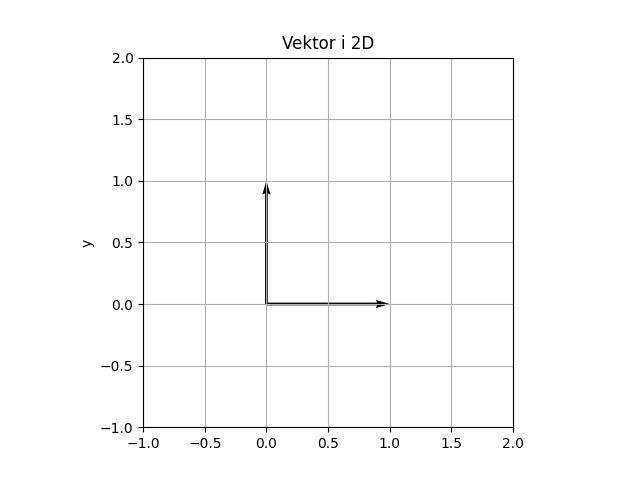
\includegraphics[width=0.6\linewidth]{Figs/ortogonalt1.png}
    \caption{En enkel vektor $\vec{b_1} = (1,0), \vec{b_2} = (0,1)$ tegnet fra origo.}
    \label{fig:vector1}
\end{figure}

\subsubsection{Plott for basis 2}

Her ser du en figur av listen $ \mathcal{C} = \left( c_1, c_2 \right)  $. Vi kan se at vektorene er ortogonale fordi de står vinkelrett på hverandre


\begin{figure}[H]
    \centering
    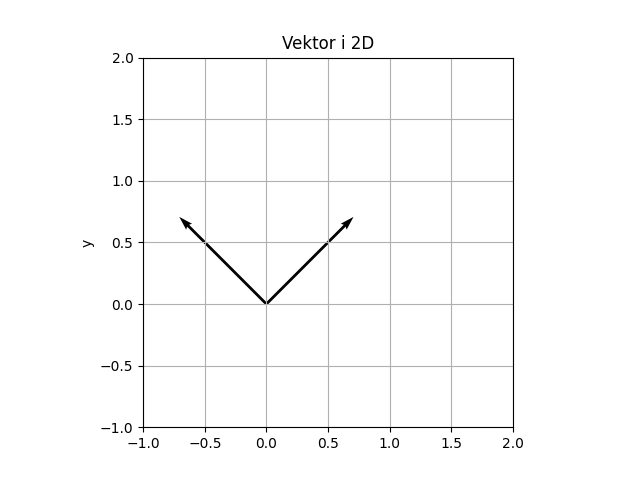
\includegraphics[width=0.6\linewidth]{Figs/ortogonalt2.png}
    \caption{En enkel vektor $\vec{c_1} = ( \frac{1} { \sqrt{ 2 }}  ,\frac{1} { \sqrt{ 2 }} ), \vec{c_2} = ( -\frac{1} { \sqrt{ 2 }}, \frac{1} { \sqrt{ 2 }})$ tegnet fra origo.}
    \label{fig:vector1}
\end{figure}

\subsubsection{Beregning av ortogonale vektorer}


Det er ganske lett og finne ut av at disse er ortogonale

\begin{enumerate}
    \item $ \mathcal{B}= \left( \begin{pmatrix}
        1 \\
        0
    \end{pmatrix}, \begin{pmatrix}
        0 \\
        1
    \end{pmatrix}  \right) = \left( b_1, b_2 \right)  $ 
    \item $ \mathcal{C}= \left( \begin{pmatrix}
        1 / \sqrt{ 2 } \\
        1 / \sqrt{ 2 }
    \end{pmatrix}, \begin{pmatrix}
        -1 / \sqrt{ 2 } \\
        1 / \sqrt{ 2 }
    \end{pmatrix}  \right) = \left( c_1, c_2 \right)  $
\end{enumerate}

\begin{align*}
    \langle b_1, b_2 \rangle_{  } = 1*0 + 0*1 = 0 \\
    \langle c_1, c_2 \rangle_{  } = \frac{ 1 }{ \sqrt{ 2 } } * \frac{ -1 }{ \sqrt{ 2 } } + \frac{ 1 }{ \sqrt{ 2 } } * \frac{ 1 }{ \sqrt{ 2 } } \\
    = \frac{ -1 }{ 2 } + \frac{ 1 }{ 2 } = 0
\end{align*}

Så begge listene $ \mathcal{B} $ og $ \mathcal{C} $ er ortogonale  



\subsection{4.3.3}

\begin{solbox}
    Vet at en liste med vektorer $ \left( u_1, ..., u_n \right) $ er lin. uavh. om 
    
    \[
        0 = \sum_{ k=1 }^{ n } \alpha_{k}^{} u_k
    \]
    har eneste løsning at $ \alpha_{1}^{} =...= \alpha_{n}^{} =0 $ 
    
    Vi setter $ \alpha_{j}^{} = \langle u_j, u_k \rangle_{  } \forall j\neq k$. Hvis vi plukker en vilkårlig u med i $ \left( u_1, ..., u_n \right) $ så har vi at 
    
    \begin{align*}
        \alpha_{j}^{} u_j &= \langle u_j, u_k \rangle_{  } u_j \\
    \end{align*}

    Og siden $ \left( u_1, ..., u_n \right) $ er ortogonal, så er $ \alpha_{j}^{} = 0 \forall j\neq k $. Så vi får bare at
    
    \[
        \alpha_{j}^{} u_j = \langle u_j, u_j \rangle_{  } u_j
    \]

    Og listen $ \left( u_1, ..., u_n \right)  $ er lin. uavh. automatisk av ortogonalitet 
    
    
\end{solbox}

\end{document}
